\section{Colored Graphs}

In this section, I will explain my model of computation which I call Colored Graphs.
It consists of a simple (undirected, no multi-edges, no loops) graph $G = (V, E)$,
together with an edge coloring $c : E \to \C$ that assigns each edge a color from a finite set of Colors $\C$.
You can find an example of a graph below.

\begin{figure}[H]
    \label{fig:graph1}
    \centering
    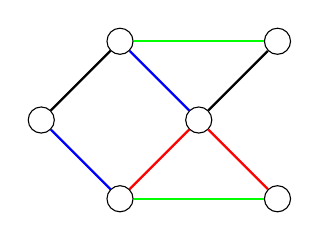
\begin{tikzpicture}
        \node[circle,draw] (A) at (1,-1) {};
        \node[circle,draw] (B) at (2,0) {};
        \node[circle,draw] (C) at (1,1) {};
        \node[circle,draw] (D) at (3,1) {};
        \node[circle,draw] (E) at (3,-1) {};
        \node[circle,draw] (F) at (0,0) {};
        
        \draw[red, thick] (A) -- (B);
        \draw[blue, thick] (B) -- (C);
        \draw[green, thick] (C) -- (D);
        \draw[black, thick] (B) -- (D);
        \draw[green, thick] (E) -- (A);
        \draw[blue, thick] (F) -- (A);
        \draw[black, thick] (F) -- (C);
        \draw[red, thick] (B) -- (E);
    \end{tikzpicture}
    \caption{Example of a Colored Graph}
\end{figure}


The model computes by applying rules to the vertices of a graph which I will first describe informally.
To determine whether a rule can be applied to a vertex of the graph, we look at the colors of incident edges to that vertex.
Concretely, an example rule might apply when a node is incident to 2 red edges and 1 black edge.
When a rule is being applied to a vertex, it changes the graph.
This, however, can not happen in an arbitrary way, but only in two simple ways.
First, the rule can delete the vertex and "rewire" the adjacent vertices, or secondly it can split the vertex in two independent nodes and connected the two vertices to the adjacent vertices of the original vertex.
Next I will describe the rules more formally.

\paragraph*{Delete Rule} A Delete Rule has a condition $b : \C \to \N$.
We say this rule can be applied to a vertex $v$ if the vertex has exactly $b(c)$ incident edges of color $c$ for all $c \in \C$.
If a Delete Rule is applied, the vertex $v$ is deleted and the adjacent vertices rewired.
Since the rule does not distinguish between different neighboring vertices nor different edges of the same color, the rewiring will be of the form "connect the vertices of the blue edges to the vertices of the red edges with a new yellow edge".
Or more formally we have a mapping $d: \C \times \C \rightharpoonup C$, that maps some pairs of colors to a new color.
Note that this in particular also allows a pair of the same color to be mapped to a new color.
This behaves basically in the same way as two different colors, by connecting all vertices connected by this color to each other.
However, no loops will be created, so vertices are not connected to themselves in that case.
In case the Delete Rule connects two vertices that are already connected, the new edge "overwrites" the old edge.

Instead of defining rules completely formally, I will mostly show them visually in the following way where the node the rule is applied to is marked in black.

\begin{center}
    \begin{tikzpicture}
    \begin{scope}[xshift=-2cm]
        \node[circle,draw] (A) at (1,-1) {};
        \node[circle,draw,fill] (B) at (2,0) {};
        \node[circle,draw] (C) at (1,1) {};
        \node[circle,draw] (D) at (3,1) {};
        \node[circle,draw] (E) at (3,-1) {};
        
        \draw[red, thick] (A) -- (B);
        \draw[blue, thick] (B) -- (C);
        \draw[black, thick] (B) -- (D);
        \draw[red, thick] (B) -- (E);
    \end{scope}

    \draw [line width=1pt, double distance=3pt, arrows = {-Latex[length=0pt 3 0]}] (1.4,0) -- (2.5,0);
    
    \begin{scope}[xshift=2cm]
        \node[circle,draw] (A2) at (1,-1) {};
        \node[circle,draw] (C2) at (1,1) {};
        \node[circle,draw] (D2) at (3,1) {};
        \node[circle,draw] (E2) at (3,-1) {};
        
        \draw[blue, thick] (A2) -- (E2);
        \draw[yellow, thick] (A2) -- (C2);
        \draw[yellow, thick] (E2) -- (C2);
    \end{scope}
    \end{tikzpicture}
\end{center}

This represents a Delete Rule that can be applied to a node that had 2 incident red edges, one blue edge and a black edge.
After deletion of the node, it rewires the blue and red vertices with a yellow edge and the red vertices with itself with blue edges.
Notice that I will sometimes call the neighboring vertices "blue vertices" even though the vertices have no color themselves.
This is just shorthand for the vertices that are connected by a blue edge.
The rewiring of the rule above can also be formally describes as the mapping of the pairs of colors $(\text{red}, \text{blue}) \mapsto \text{yellow}$ and $(\text{red}, \text{red}) \mapsto \text{blue}$.

If we apply this rule to the middle vertex of the example graph in Figure \ref{fig:graph1}, we get the following graph.

\begin{figure}[H]
    \label{fig:graph2}
    \centering
    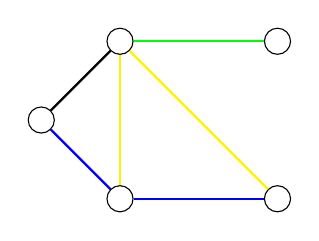
\begin{tikzpicture}
        \node[circle,draw] (A) at (1,-1) {};
        \node[circle,draw] (C) at (1,1) {};
        \node[circle,draw] (D) at (3,1) {};
        \node[circle,draw] (E) at (3,-1) {};
        \node[circle,draw] (F) at (0,0) {};
        
        \draw[green, thick] (C) -- (D);
        \draw[blue, thick] (E) -- (A);
        \draw[blue, thick] (F) -- (A);
        \draw[black, thick] (F) -- (C);
        \draw[yellow, thick] (A) -- (C);
        \draw[yellow, thick] (E) -- (C);
    \end{tikzpicture}
    \caption{Graph after applying the example Delete Rule}
\end{figure}

\paragraph*{Split Rule} A Split Rule has the same kind of condition $b : \C \to \N$ as a Delete Rule.
So again, we count the number of incident edges of each color to see if it matches the condition of the rule.
In contract to a Delete Rule, a Split Rule does not delete the vertex but splits it into two vertices.
The rule then determines which neighboring nodes the two new vertices are connected to.
Again, we don't distinguish vertices that are connected with the same color.
The new connections of the first node can we described by a mapping $s_1 : \C \rightharpoonup \C$ and the new connections of the second node by $s_2 : \C \rightharpoonup \C$.
These mapping describe the colors of the edges with which the two new vertices should be connected to some of the neighboring vertices.

An example Split Rule would be

\begin{center}
    \begin{tikzpicture}
    \begin{scope}[xshift=-2cm]
        \node[circle,draw,fill] (B) at (2,0) {};

        \node[circle,draw] (A) at (1,-1) {};
        \node[circle,draw] (C) at (2,1.3) {};
        \node[circle,draw] (E) at (3,-1) {};
        
        \draw[blue, thick] (B) -- (A);
        \draw[yellow, thick] (B) -- (C);
        \draw[blue, thick] (B) -- (E);
    \end{scope}

    \draw [line width=1pt, double distance=3pt,
             arrows = {-Latex[length=0pt 3 0]}] (1.4,0) -- (2.5,0);
    
    \begin{scope}[xshift=2cm]
        \node[circle,draw,fill] (B2) at (2.5,0) {};
        \node[circle,draw,fill] (D2) at (1.5,0) {};
        
        \node[circle,draw] (A2) at (1,-1) {};
        \node[circle,draw] (C2) at (2,1.3) {};
        \node[circle,draw] (E2) at (3,-1) {};
        
        \draw[yellow, thick] (B2) -- (C2);
        \draw[green, thick] (B2) -- (A2);
        \draw[green, thick] (B2) -- (E2);
        \draw[red, thick] (D2) -- (C2);
    \end{scope}
    
    \end{tikzpicture}
\end{center}

It represents a Split Rule that can be applied to a node that had 2 incident blue edges and one yellow edge.
The two new nodes with their new edges can be described by the mapping $s_1$ that maps yellow to red and $s_2$ which maps blue to green and yellow to yellow.

Applying this rule to the bottom left node in the graph in Figure \ref{fig:graph2}, we get the following graph.

\begin{figure}[H]
    \label{fig:graph3}
    \centering
    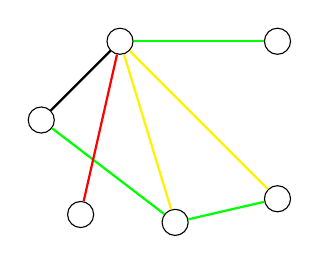
\begin{tikzpicture}
        \node[circle,draw] (A) at (1.7,-1.3) {};
        \node[circle,draw] (C) at (1,1) {};
        \node[circle,draw] (D) at (3,1) {};
        \node[circle,draw] (E) at (3,-1) {};
        \node[circle,draw] (F) at (0,0) {};
        \node[circle,draw] (G) at (0.5,-1.2) {};
        
        \draw[green, thick] (C) -- (D);
        \draw[green, thick] (E) -- (A);
        \draw[green, thick] (F) -- (A);
        \draw[black, thick] (F) -- (C);
        \draw[yellow, thick] (A) -- (C);
        \draw[yellow, thick] (E) -- (C);
        \draw[red, thick] (G) -- (C);
    \end{tikzpicture}
    \caption{Graph after applying the example Split Rule}
\end{figure}

\paragraph*{Computation}
A program in the Colored Graph model is a finite set of Delete and Split Rule.
The input to the model is an initial colored graph.
In each step of the computation an arbitrary rule is applied to a vertex that satisfies the condition of the rule.
This is repeated until no rule can be applied anymore.
Notice that this model is not necessarily confluent meaning that there might be different reductions that lead to different end results.
It is the task of the programmer to design rules and a suitable encoding of the problem input such that the computation always leads to the desired result no matter the order of rule applications.

I also implemented a simulator in Python which you can find in this GitHub repository \\
(https://github.com/nilscrm/colored-networks).
It also contains the examples that now follow.